\label{sec:Res}
\section*{Results}

Using a one-way ANOVA, we partitioned variance due to the species effect, i.e. the part of the variance explained by the species of individuals (see~\autoref{fig:aov}). Depending on the trait, the species effect could explain between 27\% up to 75\% of the variability of our data. While species effect can explain over 75\% of the variability in wood density, it only explains less than 30\% of the variability in AGR. The specific effect is strong for certain traits (wood density, toughness and SLA), but not for AGR.

Several other factors may explain residual variability: micro-environmental conditions, intra-specific variability or climatic conditions for example. In order to disentangle better the residual variance, we tested spatial auto-correlation of traits and AGR on our plots with mark correlation functions (data not shown). Neither traits nor AGR were spatially auto-correlated, i.e. the distribution of AGR or trait values in our 9 plots is not specifically distributed, indeed it is not very different from random distribution of those values in the plots. It underlines that in our data set the micro-environment does not strongly influence the traits.

From a functional point of view, the growth of individual may be explained by its traits. To test this assumption we made growth mixed-model including all selected traits of our data set (see~\autoref{tab:seltraits}) as predictors of the AGR, with both a species and a plot random effect. From previous growth model \cite{NEEDED} we knew diameter at breast height (DBH) as well as $\log(\text{DBH})$ improve AGR predictions and thus we added those two terms in our models.

An individual's trait is its species average trait plus its difference to this average. For some traits, considering the absolute distance to average trait may model better actual processes, as the important factor, in performance, is the absolute distance to species average trait. To understand whether we have to consider intra-specific variability in our data set, we compared models with individual trait value vs. models with specific trait value to which we added individual's distance measures (real or absolute); all those models were compared to the ones with only the specific trait value. We both computed models including all traits, or trait-specific models. In the end, our models predict AGR with DBH and $\log(\text{DBH})$ factors, plus species random effect both on intercept and slopes of these two factors, we added a plot intercept random effect as it improved much the R-squared of our models, and then different trait terms. \missfig (table of characteristics of models?)

The best model was the individual ones in term of R-squared. However, the model with real individual distance predicted AGR better than the one with only specific term.

We then examined the link between predicted AGR and distance to species average for each trait separately. We computed regularly spaced species average trait values in the 5\%-95\% of species average trait values in our data set as well as individual's distance to species average in the same 5\%-95\% range of values in our data set. We then associated every individual's distance to every species average trait, giving us all possible couples. From this grid of data, we predicted AGR of those simulated individuals using previous trait-specific model, using the data median DBH value. For each trait we selected the model with the highest R-squared with the lowest AIC (see~\autoref{tab:seltraits}'s last column). The best model for bark thickness had an absolute distance to species average trait term, while for all the other traits the best models were those with real (with sign) distance to species average trait.

For each trait we had AGR predictions from models for a given range of data (\autoref{fig:simul}), unraveling patterns of change in AGR with individual's distance or with species average trait. For example, AGR increases with decreasing individual's distance in SLA.

\begin{figure}[!ht]
	\centering
	\begin{subfigure}[c]{0.45\textwidth}
		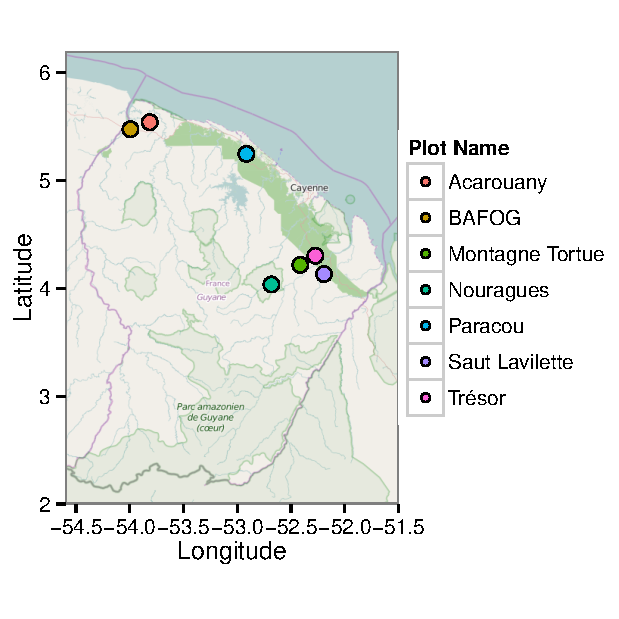
\includegraphics[scale=0.75]{figures/Plots_Map_2015-05-26.pdf}
		\caption{}
		\label{fig:map}
	\end{subfigure}
	\begin{subfigure}[c]{0.5\textwidth}
		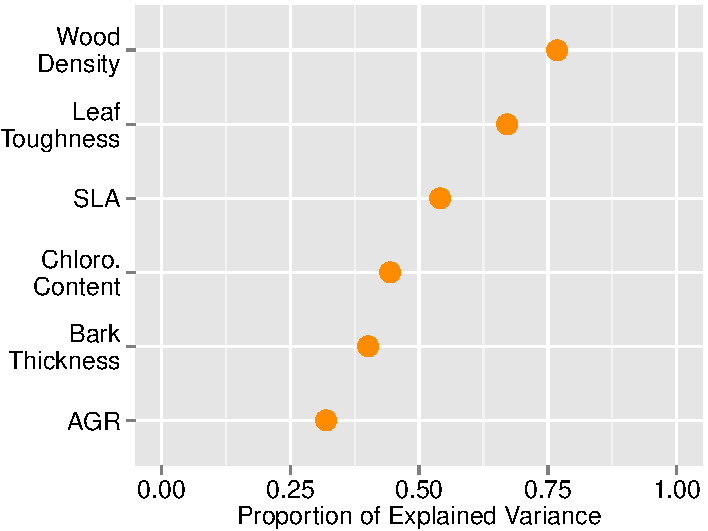
\includegraphics[scale=0.7]{figures/Aov_Var_Traits_2015-05-25.pdf}
		\caption{}
		\label{fig:aov}
	\end{subfigure}
	\caption{\textbf{(a) Plots map.} 9 1-ha plots were used, spread in French Guiana, two plots were surveyed both in Nouragues and in Paracou (see~\citealp{baraloto_decoupled_2010}) \textbf{(b) Explained variance by species effect in ANOVAs.} Dot-plot of explained variance in ANOVA by the species effect for traits and AGR. The right space after the orange is the residual variance. \textbf{Chloro. Content}: Laminar Chlorophyll Content, \textbf{AGR}: Annual Growth Rate (in diameter).}
	\label{fig:gen}
\end{figure}

\begin{figure}[!ht]
	\centering
	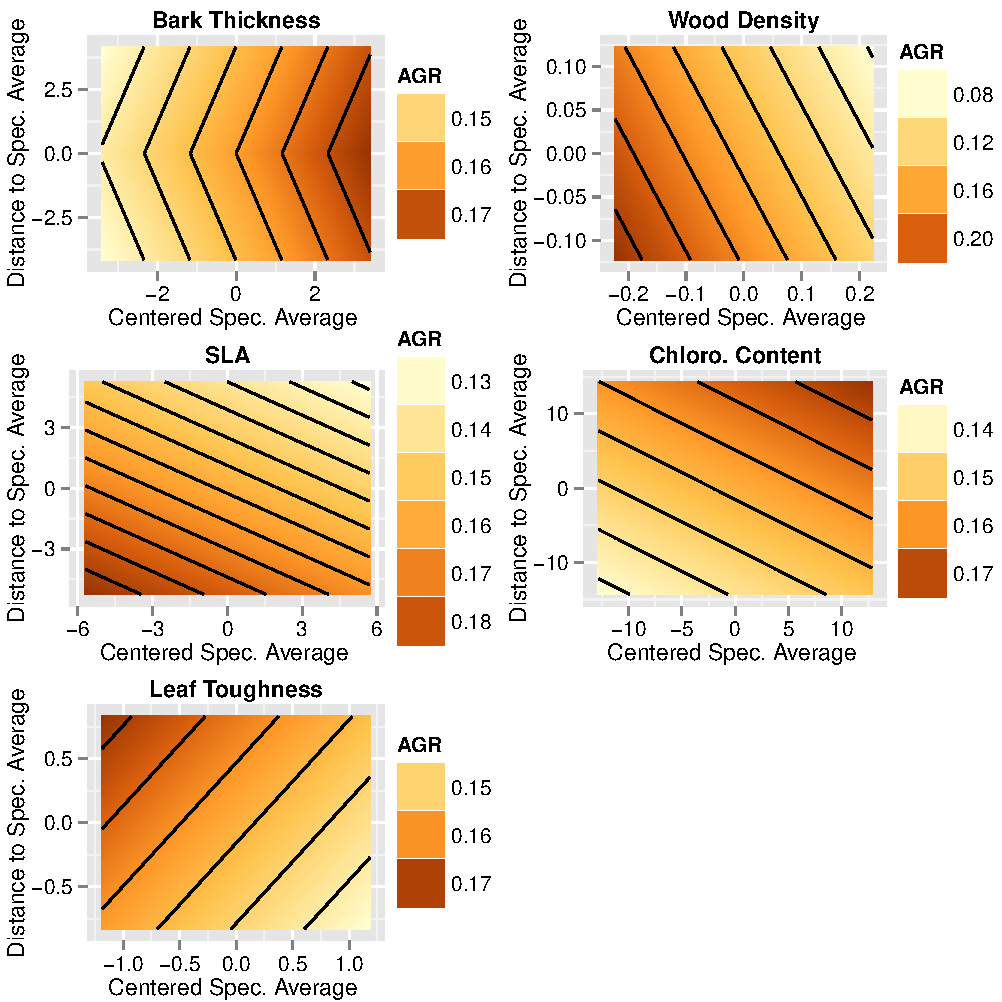
\includegraphics{figures/Sel_Traits_Simul_Pred_AGR_2015-05-22.pdf}
	\caption{\textbf{Simulations of species trait and predictions of AGR with growth models.} Surface plots of predicted AGR of simulated range of data: X-axis, centered species average trait (species average trait minus mean of all species average trait); Y-axis, individual distance to species average trait. Black lines are equal-AGR lines over the surface, i.e. on those line each point has the same AGR value. For details on traits see~\autoref{tab:seltraits}.}
	\label{fig:simul}
\end{figure}